% =====================================================================
% Segunda parte – 3. Pruebas unitarias
% =====================================================================
\section{Pruebas unitarias}

\subsection{Análisis}

Las pruebas unitarias están en \codigo{backend/tests/test_unitarias.py} (Apéndice \ref{ap:unitarias}) y se ejecutan con pytest. Importan las funciones reales del código (\codigo{app.services}, \codigo{app.scheduler} y \codigo{app.schemas}) sin servidor ni base de datos. Para cada funcionalidad aplicamos caja negra (clases de equivalencia y valores límite) y caja blanca (camino básico). Como la refactorización de la Fase A cambió la estructura de \codigo{get_date_range} y \codigo{generate_daily_amounts}, recalculamos su grafo y su complejidad sobre el código actual.

\tikzset{
  ng/.style={circle, draw, minimum size=6.5mm, inner sep=0pt, font=\scriptsize},
  ngp/.style={ng, fill=grisclaro},
  eg/.style={-{Stealth[length=1.6mm]}, thin},
  lg/.style={font=\tiny, inner sep=1pt},
}

\subsection{Funcionalidad F1: Registrar transacción}

\subsubsection{Clases de equivalencia}

\begin{table}[H]
\caption{Clases de equivalencia de F1 (\codigo{TransactionCreate})}
\label{tab:ce-f1}
\footnotesize
\begin{tabularx}{\linewidth}{L{2cm} L{3.4cm} L{1cm} Y L{1.4cm}}
\toprule
Variable & Condición & Clase & Ejemplo & Tipo \\
\midrule
amount & $0 < x \leq 9\,999\,999\,999\,999{,}99$ & CE1 & 50\,000 & Válida \\
amount & $x \leq 0$ & CE2 & 0; $-1$ & Inválida \\
amount & $x >$ máximo & CE3 & $10^{13}$ & Inválida \\
type & \{expense, income\} & CE4 & expense & Válida \\
type & Otro valor & CE5 & otro & Inválida \\
category\_id & Predeterminada o propia & CE6 & 1 & Válida \\
category\_id & Ajena o inexistente & CE7 & 999\,999 & Inválida (404) \\
frequency & Recurrente con frecuencia & CE8 & monthly & Válida \\
frequency & Recurrente sin frecuencia válida & CE9 & — & Inválida (422, D-14) \\
\bottomrule
\end{tabularx}
\tablenote{Fuente: elaboración propia.}
\end{table}

\subsubsection{Valores límite}

\begin{table}[H]
\caption{Valores límite de \codigo{amount} en F1 (\codigo{Numeric(15,2)})}
\label{tab:vl-f1}
\footnotesize
\begin{tabularx}{\linewidth}{L{3cm} L{3.4cm} L{2.2cm} Y}
\toprule
Límite & Valor & Esperado & Obtenido (antes → después) \\
\midrule
Inferior al mínimo & $-1$; 0 & 422 & 422 → 422 \\
Mínimo & 0,01 & Aceptado & Aceptado → Aceptado \\
Máximo & 9\,999\,999\,999\,999,99 & Aceptado & Aceptado → Aceptado \\
Superior al máximo & 10\,000\,000\,000\,000 & 422 & \textbf{Aceptado (D-02)} → 422 \\
\bottomrule
\end{tabularx}
\tablenote{Pruebas \codigo{test_transaccion_monto_invalido} y \codigo{test_transaccion_monto_valido}. Fuente: elaboración propia.}
\end{table}

\subsubsection{Camino básico: \texorpdfstring{\codigo{scheduler._toca_hoy}}{scheduler._toca_hoy}}

\begin{minted}[fontsize=\footnotesize, linenos, frame=single]{python}
def _toca_hoy(t, hoy: date) -> bool:
    if not t.trans_date or hoy < t.trans_date:      # nodos 1 y 2
        return False                                # nodo 14
    if t.frequency == "monthly":                    # nodo 3
        return hoy.day == t.trans_date.day          # nodo 4
    if t.frequency == "weekly":                     # nodo 5
        return hoy.weekday() == t.trans_date.weekday()   # nodo 6
    if t.frequency == "biweekly":                   # nodo 7
        return (hoy - t.trans_date).days % 14 == 0  # nodo 8
    if t.frequency == "annual":                     # nodo 9
        return hoy.day == t.trans_date.day and \
               hoy.month == t.trans_date.month      # nodos 10, 11 y 12
    return False                                    # nodo 13
\end{minted}

\begin{figure}[H]
\centering
\caption{Grafo de flujo de \codigo{_toca_hoy}}
\label{fig:grafo-toca}
\begin{tikzpicture}[node distance=7mm and 10mm]
\node[ngp] (n1) {1};
\node[ngp, below=of n1] (n2) {2};
\node[ngp, below=of n2] (n3) {3};
\node[ngp, below=of n3] (n5) {5};
\node[ngp, below=of n5] (n7) {7};
\node[ngp, below=of n7] (n9) {9};
\node[ngp, below=of n9] (n10) {10};
\node[ng, right=of n3] (n4) {4};
\node[ng, right=of n5] (n6) {6};
\node[ng, right=of n7] (n8) {8};
\node[ng, right=of n10] (n11) {11};
\node[ng, below=of n10] (n12) {12};
\node[ng, left=14mm of n9] (n13) {13};
\node[ng, left=14mm of n2] (n14) {14};
\node[ng, right=22mm of n7] (n15) {15};
\draw[eg] (n1) -- node[lg, right]{fecha} (n2);
\draw[eg] (n1) -| node[lg, above, pos=0.3]{sin fecha} (n14);
\draw[eg] (n2) -- node[lg, above]{hoy<fecha} (n14);
\draw[eg] (n2) -- (n3);
\draw[eg] (n3) -- node[lg, above]{monthly} (n4);
\draw[eg] (n3) -- (n5);
\draw[eg] (n5) -- node[lg, above]{weekly} (n6);
\draw[eg] (n5) -- (n7);
\draw[eg] (n7) -- node[lg, above]{biweekly} (n8);
\draw[eg] (n7) -- (n9);
\draw[eg] (n9) -- node[lg, right]{annual} (n10);
\draw[eg] (n9) -- node[lg, above]{otra} (n13);
\draw[eg] (n10) -- node[lg, above]{día =} (n11);
\draw[eg] (n10) -- node[lg, right]{día $\neq$} (n12);
\draw[eg] (n4) -- (n15); \draw[eg] (n6) -- (n15); \draw[eg] (n8) -- (n15); \draw[eg] (n11) -- (n15);
\draw[eg] (n12) -| (n15);
\draw[eg] (n13) |- ([yshift=-14mm]n12.south) -| (n15);
\draw[eg] (n14) |- ([yshift=8mm]n1.north) -| (n15);
\end{tikzpicture}
\figurenote{Los nodos grises son predicados. Fuente: elaboración propia.}
\end{figure}

\paragraph{Complejidad ciclomática.} El grafo tiene $A = 21$ aristas y $N = 15$ nodos: $V(G) = A - N + 2 = 21 - 15 + 2 = 8$. Con los siete nodos predicado (1, 2, 3, 5, 7, 9 y 10), $V(G) = P + 1 = 8$. La herramienta de métricas (Tercera parte) mide también 8. Se necesitan 8 caminos independientes.

\begin{table}[H]
\caption{Caminos independientes de \codigo{_toca_hoy} (fecha de origen: 31/01/2026)}
\label{tab:caminos-toca}
\footnotesize
\begin{tabularx}{\linewidth}{L{0.8cm} L{3.3cm} L{3.4cm} L{1.4cm} Y}
\toprule
Camino & Secuencia & Datos (frecuencia, hoy) & Esperado & Obtenido \\
\midrule
C1 & 1-14-15 & sin fecha de origen & False & False \\
C2 & 1-2-14-15 & monthly, 01/01/2026 & False & False \\
C3 & 1-2-3-4-15 & monthly, 31/03/2026 & True & True \\
C4 & 1-2-3-5-6-15 & weekly, 07/02/2026 & True & True \\
C5 & 1-2-3-5-7-8-15 & biweekly, 14/02/2026 & True & True \\
C6 & 1-2-3-5-7-9-10-11-15 & annual, 31/01/2027 & True & True \\
C7 & 1-2-3-5-7-9-10-12-15 & annual, 28/02/2027 & False & False \\
C8 & 1-2-3-5-7-9-13-15 & otra, 31/03/2026 & False & False \\
\bottomrule
\end{tabularx}
\tablenote{Pruebas \codigo{test_toca_hoy} (parametrizada) y \codigo{test_toca_hoy_sin_fecha}. Fuente: elaboración propia.}
\end{table}

\subsection{Funcionalidad F2: Gestionar presupuesto}

\subsubsection{Clases de equivalencia}

\begin{table}[H]
\caption{Clases de equivalencia de F2 (\codigo{BudgetCreate})}
\label{tab:ce-f2}
\footnotesize
\begin{tabularx}{\linewidth}{L{2.2cm} L{3.6cm} L{1cm} Y L{1.4cm}}
\toprule
Variable & Condición & Clase & Ejemplo & Tipo \\
\midrule
amount & $0 < x \leq$ máximo & CE1 & 600\,000 & Válida \\
amount & $x \leq 0$ & CE2 & 0 & Inválida \\
period\_type & \{daily, weekly, monthly, unique\} & CE3 & monthly & Válida \\
period\_type & Otro & CE4 & yearly & Inválida \\
month & $1 \leq m \leq 12$ & CE5 & 11 & Válida \\
month & $m < 1$ o $m > 12$ & CE6 & 13 & Inválida \\
year & $2000 \leq a \leq 2100$ & CE7 & 2026 & Válida \\
year & Fuera del rango & CE8 & 1999 & Inválida \\
Período único & inicio $\leq$ fin & CE9 & 01/11 a 30/11 & Válida \\
Período único & inicio $>$ fin o sin fechas & CE10 & 01/02 a 01/01 & Inválida \\
\bottomrule
\end{tabularx}
\tablenote{Fuente: elaboración propia.}
\end{table}

\subsubsection{Valores límite}

\begin{table}[H]
\caption{Valores límite de F2}
\label{tab:vl-f2}
\footnotesize
\begin{tabularx}{\linewidth}{L{2.6cm} L{3.6cm} L{2.6cm} Y}
\toprule
Límite & Valor & Esperado & Obtenido (antes → después) \\
\midrule
Mes inferior & month = 0 & 422 & \textbf{Aceptado} → 422 \\
Mes mínimo y máximo & month = 1; 12 & Aceptado & Aceptado → Aceptado \\
Mes superior & month = 13 & 422 & \textbf{500 (D-03)} → 422 \\
Febrero bisiesto & 2/2028 & 01/02 a 29/02 & Igual → Igual \\
Porcentaje & gasto 120, límite 100 & 120\,\% & \textbf{100\,\% (D-04)} → 120\,\% \\
\bottomrule
\end{tabularx}
\tablenote{Pruebas \codigo{test_presupuesto_mes_invalido}, \codigo{test_presupuesto_mes_limite_valido}, \codigo{test_rango_mensual_valores_limite} y \codigo{test_pi04_d04_porcentaje_supera_100}. Fuente: elaboración propia.}
\end{table}

\subsubsection{Camino básico: cálculo del período mensual}

Tras la refactorización, \codigo{get_date_range} solo elige la función del período en un diccionario ($V(G) = 3$); la lógica con decisiones quedó en \codigo{_monthly_range}, que analizamos:

\begin{minted}[fontsize=\footnotesize, linenos, frame=single]{python}
def _monthly_range(budget, today: date) -> tuple:
    use_today = budget.is_permanent
    month = today.month if use_today or not budget.month else budget.month   # nodos 1-4
    year = today.year if use_today or not budget.year else budget.year       # nodos 5-8
    return date(year, month, 1), date(year, month, calendar.monthrange(year, month)[1])  # nodo 9
\end{minted}

\begin{figure}[H]
\centering
\caption{Grafo de flujo de \codigo{_monthly_range}}
\label{fig:grafo-mensual}
\begin{tikzpicture}[node distance=7mm and 12mm]
\node[ngp] (m1) {1};
\node[ngp, below right=of m1] (m2) {2};
\node[ng, below left=of m2] (m3) {3};
\node[ng, below right=of m2] (m4) {4};
\node[ngp, below=16mm of m2] (m5) {5};
\node[ngp, below right=of m5] (m6) {6};
\node[ng, below left=of m6] (m7) {7};
\node[ng, below right=of m6] (m8) {8};
\node[ng, below=16mm of m6] (m9) {9};
\draw[eg] (m1) -- node[lg, left]{permanente} (m3);
\draw[eg] (m1) -- node[lg, above right]{no} (m2);
\draw[eg] (m2) -- node[lg, above left]{sin mes} (m3);
\draw[eg] (m2) -- node[lg, above right]{con mes} (m4);
\draw[eg] (m3) -- (m5); \draw[eg] (m4) -- (m5);
\draw[eg] (m5) -- node[lg, left]{permanente} (m7);
\draw[eg] (m5) -- node[lg, above right]{no} (m6);
\draw[eg] (m6) -- node[lg, above left]{sin año} (m7);
\draw[eg] (m6) -- node[lg, above right]{con año} (m8);
\draw[eg] (m7) -- (m9); \draw[eg] (m8) -- (m9);
\end{tikzpicture}
\figurenote{Fuente: elaboración propia.}
\end{figure}

\paragraph{Complejidad ciclomática.} $V(G) = A - N + 2 = 12 - 9 + 2 = 5$, y con los predicados 1, 2, 5 y 6, $V(G) = P + 1 = 5$; coincide con la herramienta. Los nodos 1 y 5 evalúan la misma variable (\codigo{is_permanent}), por lo que los caminos que mezclan «permanente» en una decisión y «no permanente» en la otra son \textbf{no factibles}. Probamos los cuatro caminos factibles de la base y el camino C5, que es combinación lineal de C2, C3 y C4.

\begin{table}[H]
\caption{Caminos de \codigo{_monthly_range} (hoy = 21/11/2026)}
\label{tab:caminos-mensual}
\footnotesize
\begin{tabularx}{\linewidth}{L{0.8cm} L{2.8cm} L{3.6cm} Y L{1.4cm}}
\toprule
Camino & Secuencia & Datos & Esperado & Obtenido \\
\midrule
C1 & 1-3-5-7-9 & permanente; mes 2/2028 & 01/11/2026 a 30/11/2026 & Igual \\
C2 & 1-2-4-5-6-8-9 & mes 2, año 2028 & 01/02/2028 a 29/02/2028 & Igual \\
C3 & 1-2-3-5-6-8-9 & sin mes, año 2027 & 01/11/2027 a 30/11/2027 & Igual \\
C4 & 1-2-4-5-6-7-9 & mes 4, sin año & 01/04/2026 a 30/04/2026 & Igual \\
C5 & 1-2-3-5-6-7-9 & sin mes ni año & 01/11/2026 a 30/11/2026 & Igual \\
\bottomrule
\end{tabularx}
\tablenote{Prueba \codigo{test_camino_basico_rango_mensual}; los demás períodos se cubren con \codigo{test_rango_*}. Fuente: elaboración propia.}
\end{table}

\subsection{Funcionalidad F3: Gestionar meta de ahorro}

\subsubsection{Clases de equivalencia}

\begin{table}[H]
\caption{Clases de equivalencia de F3 (\codigo{SavingGoalCreate} y \codigo{useMetaForm})}
\label{tab:ce-f3}
\footnotesize
\begin{tabularx}{\linewidth}{L{2.4cm} L{3.4cm} L{1cm} Y L{1.6cm}}
\toprule
Variable & Condición & Clase & Ejemplo & Tipo \\
\midrule
name & No vacío tras quitar espacios & CE1 & Viaje & Válida \\
name & Vacío o solo espacios & CE2 & «   » & Inválida \\
target\_amount & $> 0$ y múltiplo de 1000 & CE3 & 300\,000 & Válida \\
target\_amount & $\leq 0$ & CE4 & 0 & Inválida \\
target\_amount & $> 0$ no múltiplo de 1000 & CE5 & 1\,500 & Inválida (cliente) \\
end\_date & $\geq$ hoy & CE6 & hoy + 29 & Válida \\
end\_date & $<$ hoy & CE7 & ayer & Inválida \\
end\_date & Ausente & CE8 & — & Válida (30 días) \\
Fechas & inicio $>$ fin & CE9 & +10 y +1 días & Inválida \\
\bottomrule
\end{tabularx}
\tablenote{Fuente: elaboración propia.}
\end{table}

\subsubsection{Valores límite}

\begin{table}[H]
\caption{Valores límite de F3}
\label{tab:vl-f3}
\footnotesize
\begin{tabularx}{\linewidth}{L{3.2cm} L{3.4cm} L{3cm} Y}
\toprule
Límite & Valor & Esperado & Obtenido (antes → después) \\
\midrule
Fecha inferior & end\_date = ayer & 422 & 422 → 422 \\
Duración mínima & 1 día, 50\,000 & \{1: 50\,000\} & Igual → Igual \\
Dos días & 2 días, 1\,000 COP & Suma 1\,000, cuotas $\geq 0$ & Igual → Igual \\
Objetivo $<$ días × unidad & 15 días, 1\,000 COP & Cuotas $\geq 0$, suma 1\,000 & \textbf{día 15 = $-400$ (D-01)} → 10 × 100 y 5 × 0 \\
Sin fecha final & end\_date ausente & 31 cuotas & \textbf{500 (D-07)} → 31 cuotas \\
\bottomrule
\end{tabularx}
\tablenote{Pruebas \codigo{test_plan_suma_objetivo_y_sin_negativos}, \codigo{test_d01_caso_reportado_1000_en_15_dias} y \codigo{test_pi10_d07_meta_sin_fecha_final}. Fuente: elaboración propia.}
\end{table}

\subsubsection{Camino básico: \texorpdfstring{\codigo{saving_service.generate_daily_amounts}}{saving_service.generate_daily_amounts}}

\begin{minted}[fontsize=\footnotesize, linenos, frame=single]{python}
def generate_daily_amounts(start_date, end_date, target_amount, currency=DEFAULT_CURRENCY):
    end_date = end_date or start_date + timedelta(days=DEFAULT_DURATION_DAYS)  # nodos 1-3
    num_days = (end_date - start_date).days + 1
    if num_days <= 0:                                                         # nodo 3
        raise ValueError("La fecha de fin debe ser después de la fecha de inicio")  # nodo 4
    target = float(target_amount)
    min_unit = get_min_unit(currency)
    if num_days == 1:                                                         # nodo 5
        return {"1": round_to_unit(target, min_unit)}                         # nodo 6
    if target < num_days * min_unit:                                          # nodo 7
        return _distribute_insufficient(target, num_days, min_unit)           # nodo 8
    return _distribute_variable(target, num_days, min_unit)                   # nodo 9
\end{minted}

\begin{figure}[H]
\centering
\caption{Grafo de flujo de \codigo{generate_daily_amounts}}
\label{fig:grafo-plan}
\begin{tikzpicture}[node distance=7mm and 12mm]
\node[ngp] (g1) {1};
\node[ng, right=of g1] (g2) {2};
\node[ngp, below=of g1] (g3) {3};
\node[ng, right=of g3] (g4) {4};
\node[ngp, below=of g3] (g5) {5};
\node[ng, right=of g5] (g6) {6};
\node[ngp, below=of g5] (g7) {7};
\node[ng, right=of g7] (g8) {8};
\node[ng, below=of g7] (g9) {9};
\node[ng, right=32mm of g7] (g10) {10};
\draw[eg] (g1) -- node[lg, above]{sin fin} (g2);
\draw[eg] (g1) -- (g3);
\draw[eg] (g2) -- (g3);
\draw[eg] (g3) -- node[lg, above]{$\leq 0$} (g4);
\draw[eg] (g3) -- (g5);
\draw[eg] (g5) -- node[lg, above]{= 1} (g6);
\draw[eg] (g5) -- (g7);
\draw[eg] (g7) -- node[lg, above]{insuf.} (g8);
\draw[eg] (g7) -- node[lg, left]{normal} (g9);
\draw[eg] (g4) -| (g10); \draw[eg] (g6) -| (g10); \draw[eg] (g8) -- (g10); \draw[eg] (g9) -| (g10);
\end{tikzpicture}
\figurenote{Fuente: elaboración propia.}
\end{figure}

\paragraph{Complejidad ciclomática.} $V(G) = A - N + 2 = 13 - 10 + 2 = 5$; con los predicados 1, 3, 5 y 7, $V(G) = P + 1 = 5$. Antes de la refactorización la función tenía $V(G) = 7$ y dos bucles; ahora el reparto está en \codigo{_distribute_insufficient} y \codigo{_distribute_variable}, que se prueban a través de los caminos C4 y C5.

\begin{table}[H]
\caption{Caminos independientes de \codigo{generate_daily_amounts}}
\label{tab:caminos-plan}
\footnotesize
\begin{tabularx}{\linewidth}{L{0.8cm} L{2.4cm} L{3.6cm} Y}
\toprule
Camino & Secuencia & Datos & Resultado (después) \\
\midrule
C1 & 1-2-3-5-7-9-10 & 01/01/2026, sin fin, 310\,000 & 31 cuotas, suma 310\,000 (aprobado) \\
C2 & 1-3-4-10 & fin anterior al inicio & \codigo{ValueError} (aprobado) \\
C3 & 1-3-5-6-10 & 1 día, 50\,000 & \{1: 50\,000\} (aprobado) \\
C4 & 1-3-5-7-8-10 & 15 días, 1\,000 COP & 10 cuotas de 100 y 5 de 0 (aprobado; antes: $-400$, D-01) \\
C5 & 1-3-5-7-9-10 & 30 días, 300\,000 COP & 30 cuotas múltiplos de 100, suma 300\,000 (aprobado) \\
\bottomrule
\end{tabularx}
\tablenote{Pruebas \codigo{test_plan_*} y \codigo{test_d01_*}; \codigo{test_plan_es_determinista} verifica además que la semilla produce siempre el mismo plan. Fuente: elaboración propia.}
\end{table}

\subsection{Diseño de casos de prueba}

{\footnotesize\renewcommand{\arraystretch}{1.2}
\begin{longtable}{L{1.8cm} L{0.9cm} L{3.2cm} L{6.6cm} L{1cm}}
\caption{Casos de prueba unitarios y su prueba automatizada}\label{tab:cpu}\\
\toprule
ID & Func. & Técnica y clase & Prueba en \codigo{test_unitarias.py} & Casos \\
\midrule
\endfirsthead
\toprule
ID & Func. & Técnica y clase & Prueba en \codigo{test_unitarias.py} & Casos \\
\midrule
\endhead
\bottomrule
\endfoot
CPU-01–03 & F1 & CE2, CE3; VL & \codigo{test_transaccion_monto_invalido} & 3 \\
CPU-04–06 & F1 & CE1; VL & \codigo{test_transaccion_monto_valido} & 3 \\
CPU-07 & F1 & CE5 & \codigo{test_transaccion_tipo_invalido} & 1 \\
CPU-08–18 & F1 & Camino básico C1–C8 & \codigo{test_toca_hoy}, \codigo{test_toca_hoy_sin_fecha} & 11 \\
CPU-19–21 & F2 & CE6; VL & \codigo{test_presupuesto_mes_invalido} & 3 \\
CPU-22–23 & F2 & CE5; VL & \codigo{test_presupuesto_mes_limite_valido} & 2 \\
CPU-24 & F2 & CE10 & \codigo{test_presupuesto_unico_exige_fechas_ordenadas} & 1 \\
CPU-25–29 & F2 & VL (meses de 28 a 31 días) & \codigo{test_rango_mensual_valores_limite} & 5 \\
CPU-30–34 & F2 & Camino básico C1–C5 & \codigo{test_camino_basico_rango_mensual} & 5 \\
CPU-35–41 & F2 & Otros períodos & \codigo{test_rango_diario_*}, \codigo{test_rango_semanal_*}, \codigo{test_rango_mensual_permanente_*}, \codigo{test_rango_unico}, \codigo{test_rango_por_defecto} & 7 \\
CPU-42 & F3 & CE2, CE7, CE9 & \codigo{test_meta_fecha_pasada_y_orden} & 1 \\
CPU-43–50 & F3 & VL y caminos C3–C5 & \codigo{test_plan_suma_objetivo_y_sin_negativos} & 8 \\
CPU-51 & F3 & Camino C4 (D-01) & \codigo{test_d01_caso_reportado_1000_en_15_dias} & 1 \\
CPU-52 & F3 & Determinismo & \codigo{test_plan_es_determinista} & 1 \\
CPU-53 & F3 & Camino C2 & \codigo{test_plan_fecha_fin_anterior_lanza_error} & 1 \\
CPU-54 & F3 & Camino C1 & \codigo{test_plan_sin_fecha_fin_usa_31_dias} & 1 \\
CPU-55 & F3 & Progreso & \codigo{test_calculate_progress} & 1 \\
CPU-56–58 & F1 & CE9 (D-14) & \codigo{test_d14_recurrente_exige_frecuencia_valida} & 3 \\
\midrule
\multicolumn{4}{l}{Total} & 58 \\
\end{longtable}
}
\vspace{-1em}
{\small\textit{Nota.} Fuente: elaboración propia.}

\subsection{Ejecución y evaluación}

Las pruebas se ejecutan desde \codigo{backend/} con \codigo{python -m pytest --cov=app}. La salida completa de la segunda ejecución está en \codigo{docs/reporte_cobertura.txt}; su resumen es:

\begin{minted}[fontsize=\footnotesize, frame=single]{text}
tests/test_unitarias.py ....................................... 58 passed
tests/test_integracion.py ..................................... 39 passed
TOTAL   879 sentencias   41 sin cubrir   95 % de cobertura
97 passed in 29.74s
\end{minted}

\begin{figure}[H]
\centering
\caption{Reporte de cobertura de pytest-cov (segunda ejecución)}
\label{fig:cobertura}
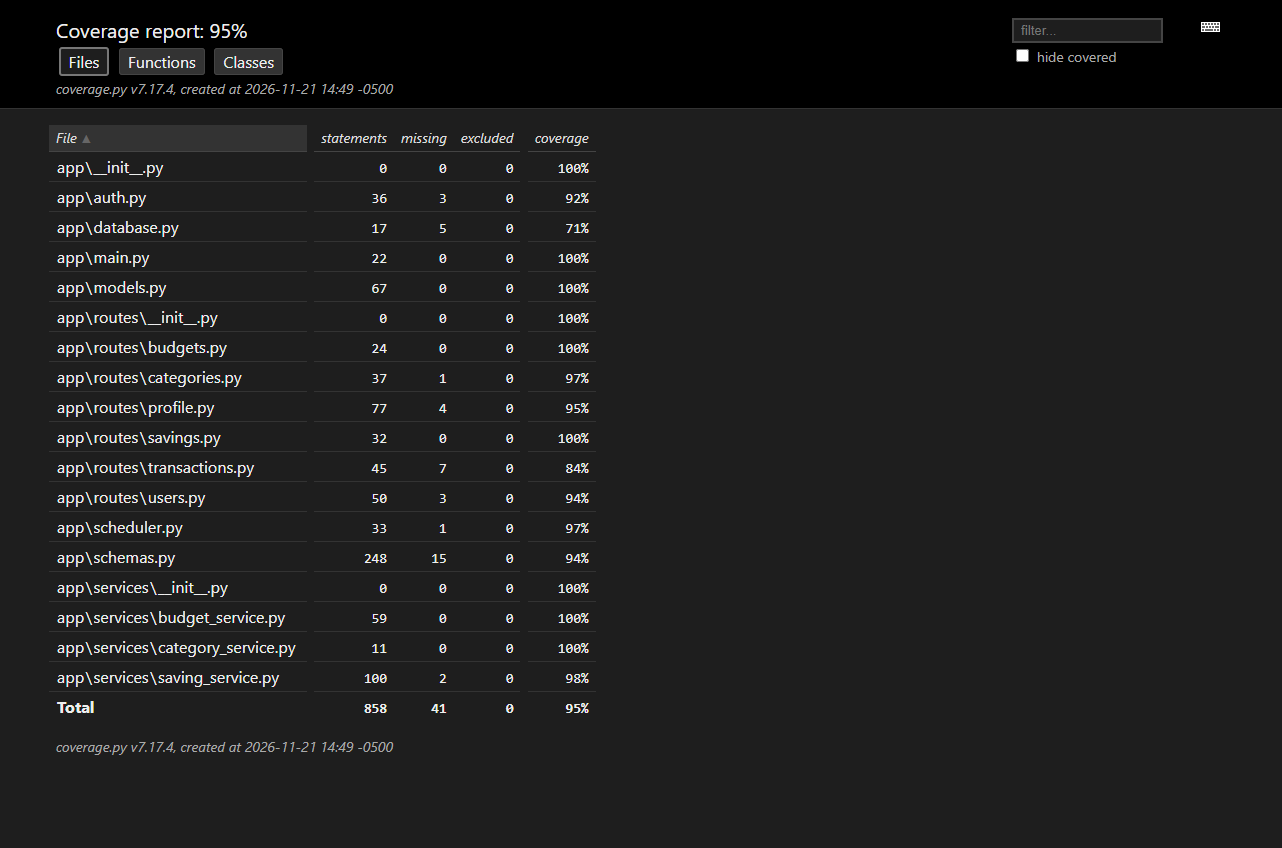
\includegraphics[width=0.85\linewidth]{../evidencias/cobertura_html.png}
\figurenote{Fuente: elaboración propia con coverage.py 7.17.4.}
\end{figure}

\begin{table}[H]
\caption{Evaluación de las pruebas unitarias}
\label{tab:eval-unitarias}
\footnotesize
\begin{tabularx}{\linewidth}{L{4cm} Y Y}
\toprule
Medida & Primera ejecución (25/10/2026) & Segunda ejecución (21/11/2026) \\
\midrule
Casos ejecutados & 49 (unittest, código extraído con \codigo{ast}) & 58 (pytest sobre los módulos reales) \\
Aprobados & 48 (98,0\,\%) & 58 (100\,\%) \\
Fallidos & 1 (D-01) & 0 \\
Defectos documentados & D-01, D-02, D-03 & Corregidos y verificados \\
Cobertura de caminos (3 métodos) & 100\,\% de los caminos de la base & 100\,\% de los caminos factibles \\
Cobertura de líneas del backend & No medida (0\,\% en SonarQube) & 95\,\% (unitarias + integración) \\
\bottomrule
\end{tabularx}
\tablenote{Fuente: elaboración propia.}
\end{table}

\paragraph{Conclusión.} Todas las pruebas unitarias pasan y la cobertura del backend (95\,\%) supera el objetivo de RNF09 (80\,\%). Los módulos de reglas de negocio (\codigo{budget_service}, \codigo{saving_service} y \codigo{category_service}) tienen entre 98 y 100\,\% de cobertura. La caja blanca encontró el defecto D-01, que la validación del cliente no prevenía, y la caja negra encontró las validaciones ausentes D-02 y D-03; las tres quedaron corregidas y cubiertas por pruebas que fallaban antes del cambio y pasan después.
